%%%%%%%%%%%%%%%%%% PREAMBULE %%%%%%%%%%%%%%%%%%

\documentclass[11pt,a4paper]{article}

\usepackage{amsfonts,amsmath,amssymb,amsthm}
\usepackage[utf8]{inputenc}
\usepackage[T1]{fontenc}
\usepackage[french]{babel}
\usepackage{fancybox}
\usepackage{graphicx}
%\usepackage{tikz}

%----- Ensembles : entiers, reels, complexes -----
\newcommand{\Nn}{\mathbb{N}} \newcommand{\N}{\mathbb{N}}
\newcommand{\Zz}{\mathbb{Z}} \newcommand{\Z}{\mathbb{Z}}
\newcommand{\Qq}{\mathbb{Q}} \newcommand{\Q}{\mathbb{Q}}
\newcommand{\Rr}{\mathbb{R}} \newcommand{\R}{\mathbb{R}}
\newcommand{\Cc}{\mathbb{C}} \newcommand{\C}{\mathbb{C}}
\newcommand{\Kk}{\mathbb{K}} \newcommand{\K}{\mathbb{K}}

%----- Modifications de symboles -----
\renewcommand{\epsilon}{\varepsilon}
\renewcommand{\Re}{\mathop{\mathrm{Re}}\nolimits}
\renewcommand{\Im}{\mathop{\mathrm{Im}}\nolimits}
\newcommand{\llbracket}{\left[\kern-0.15em\left[}
\newcommand{\rrbracket}{\right]\kern-0.15em\right]}
\renewcommand{\ge}{\geqslant} \renewcommand{\geq}{\geqslant}
\renewcommand{\le}{\leqslant} \renewcommand{\leq}{\leqslant}

%----- Fonctions usuelles -----
\newcommand{\ch}{\mathop{\mathrm{ch}}\nolimits}
\newcommand{\sh}{\mathop{\mathrm{sh}}\nolimits}
\renewcommand{\tanh}{\mathop{\mathrm{th}}\nolimits}
\newcommand{\cotan}{\mathop{\mathrm{cotan}}\nolimits}
\newcommand{\Arcsin}{\mathop{\mathrm{arcsin}}\nolimits}
\newcommand{\Arccos}{\mathop{\mathrm{arccos}}\nolimits}
\newcommand{\Arctan}{\mathop{\mathrm{arctan}}\nolimits}
\newcommand{\Argsh}{\mathop{\mathrm{argsh}}\nolimits}
\newcommand{\Argch}{\mathop{\mathrm{argch}}\nolimits}
\newcommand{\Argth}{\mathop{\mathrm{argth}}\nolimits}
\newcommand{\pgcd}{\mathop{\mathrm{pgcd}}\nolimits} 

%----- Structure des exercices ------
%\theoremstyle{definition}

\newtheoremstyle{exostyle}
{15pt}
{15pt}
{\normalfont}
{0pt}
{\bfseries}
{}
{\newline}
{\thmname{#1}~\thmnumber{#2} -- \thmnote{#3}}
\theoremstyle{exostyle} 

\newtheorem{exo}{Exercice}
\newtheorem{ind}{Indications}
\newtheorem{cor}{Correction}

\newcommand{\exercice}[1]{} \newcommand{\finexercice}{}
%\newcommand{\exercice}[1]{{\tiny\texttt{#1}}\vspace{-2ex}} % pour afficher le numero absolu, l'auteur...
\newcommand{\enonce}{\begin{exo}} \newcommand{\finenonce}{\end{exo}}
\newcommand{\indication}{\begin{ind}} \newcommand{\finindication}{\end{ind}}
\newcommand{\correction}{\begin{cor}} \newcommand{\fincorrection}{\end{cor}}

\newcommand{\noindication}{\stepcounter{ind}}
\newcommand{\nocorrection}{\stepcounter{cor}}

\newcommand{\fiche}[1]{} \newcommand{\finfiche}{}
\newcommand{\titre}[1]{\centerline{\large \bf #1}}
\newcommand{\addcommand}[1]{}
\newcommand{\video}[1]{}

%----- Presentation ------
\setlength{\parindent}{0cm}

\newcommand{\ExoSept}{\textbf{\textsf{Exo7}}}
\newcommand{\LogoExoSept}{\setlength{\unitlength}{0.6em}
	\begin{picture}(0,0)  \thicklines     \put(0,4){\line(0,1){3}}   \put(0,7){\line(1,0){3}}
		\put(3,7){\line(0,-1){7}}  \put(0,4){\line(1,0){7}}   \put(3,0){\line(1,0){4}}
		\put(7,0){\line(0,1){4}}   \put(3,7){\line(4,-3){4}}  \put(7,4){\line(3,4){3}}  
		\put(10,8){\line(-4,3){4}} \put(3,7){\line(3,4){3}}   \put(4.6,6.8){\mbox{\ExoSept}}
\end{picture}}

%----- Commandes supplementaires ------

\usepackage[a4paper, margin = 2cm]{geometry}
\usepackage[charter]{mathdesign}
%\usepackage{import}

\usepackage{tikz}
\usetikzlibrary{calc,shadows,arrows,shapes,patterns,matrix}
\usetikzlibrary{decorations.pathmorphing}
\usetikzlibrary{fadings}
\usetikzlibrary{external}
\usetikzlibrary{positioning}
\usetikzlibrary{arrows}
\usetikzlibrary{backgrounds}
\usepackage{tikz,tikz-3dplot}

\newcommand{\sauteligne}{\leavevmode\vspace{-\baselineskip}}

\begin{document}

	
	
%%%%%%%%%%%%%%%%%% ENTETE %%%%%%%%%%%%%%%%%%


%\kern-2em
\textsc{Feuille d'exercices 2}\hfill\textsc{Fonctions de plusieurs variables}

\vspace*{0.5ex}
\hrule\vspace*{1.5ex} 
\hfil{\textbf{\Large \textsc{Notions de topologie}}}
\vspace*{1ex} \hrule 
\vspace*{5ex} 

%===========================================
\section{Norme et produit scalaire}

% Cette fiche contient les exercices : 1740 

\exercice{}
\enonce[Produit scalaire et vecteurs]
\sauteligne
\begin{enumerate}
	\item Montrer que si $X = \left(\begin{smallmatrix}x\\y\end{smallmatrix}\right)$ et $Y = \left(\begin{smallmatrix}x'\\y'\end{smallmatrix}\right)$ sont des vecteurs de $\Rr^2$ alors
	$$\langle X \mid Y \rangle = 3xx'+ 2yy'$$ 
	définit un produit scalaire sur $\Rr^2$.
	
	\item Même question avec 
	$$\langle X \mid Y \rangle = 2xx'+ yy' + xy' + x'y.$$ 
	
	\item Soient $x,y$ et $z$ trois réels tels que 
	$x^2+y^2+z^2\leq 1$. Montrer que $(x+2y+3z)^2\leq 14$.
\end{enumerate}
\finenonce

\indication
Les trois axiomes qui définissent un produit scalaire sont : la linéarité à gauche et à droite, la symétrie et le caractère défini positif. Le principal résultat à connaître est l'inégalité de Cauchy-Schwarz.
\finindication

\correction
Rappelons les trois axiomes qui définissent un produit scalaire : la linéarité à gauche et à droite, la symétrie et le caractère défini positif. Il est plus malin de commencer par vérifier la symétrie, ainsi on aura juste à prouver la linéarité à gauche et alors la linéarité à droite en découlera.

\begin{enumerate}
	\item 
	\begin{itemize}
		\item Symétrie : $\langle Y \mid X \rangle = 3x'x+ 2y'y = \langle X \mid Y \rangle $.
		\item Linéarité à gauche, pour $\lambda,\mu\in\Rr$ : 
		\begin{align*}
		\langle \lambda X_1 + \mu X_2 \mid Y \rangle
		&= 3(\lambda x_1+\mu x_2) x'+ 2(\lambda y_1+\mu y_2)y' \\
		&= \lambda (3x_1x'+2y_1y')+\mu(3x_2x'+2y_2y') \\
		&= \lambda \langle X_1 \mid Y \rangle +\mu\langle X_2 \mid Y \rangle 
		\end{align*}
		
		\item Positivité : $\langle X \mid X \rangle = 3x^2+ 2y^2 \ge0$.
		Définie : $\langle X \mid X \rangle = 0 \iff 3x^2+ 2y^2 = 0 \iff X = (0,0)$.
	\end{itemize}
	

	\item La symétrie et la bilinéarité sont faciles à vérifier.
	
	Montrons le caractère positif :
	\[
	\langle X \mid X \rangle = 2x^2+ y^2 + 2xy = x^2 +(x+y)^2 \ge 0. \]
	Une fois écrit sous la forme de la somme de carrés, il est clair que $\langle X \mid X \rangle = 0 \iff X = (0,0)$.

	
	\item À un produit scalaire on associe une norme par la formule $\langle X \mid X \rangle = \| X \|^2$.
	L'inégalité de Cauchy-Schwarz s'écrit : $\langle X \mid Y \rangle^2 \le \| X \|^2 \| Y \|^2$.
	
	Pour cette question on considère le produit scalaire usuel de $\Rr^3$ : si $X = \left(\begin{smallmatrix}x\\y\\z\end{smallmatrix}\right)$ et $Y = \left(\begin{smallmatrix}x'\\y'\\z'\end{smallmatrix}\right)$ alors
	$\langle X \mid Y \rangle = xx'+ yy' + zz'$.
	
	On applique l'inégalité de Cauchy-Schwarz aux vecteurs $X = \left(\begin{smallmatrix}x\\y\\z\end{smallmatrix}\right)$ et $Y = \left(\begin{smallmatrix}1\\2\\3\end{smallmatrix}\right)$, ce qui donne :
	$(1\cdot x + 2\cdot y+3\cdot z)^2 \le (x^2+y^2+z^2)(1^2+2^2+3^2)$.
	Par hypothèse $x^2+y^2+z^2 \le 1$, donc $(x+2y+3z)^2 \le 14$. 
	 
\end{enumerate}
\fincorrection

\finexercice



\exercice{}
\enonce[Produit scalaire et intégrales]
Soit $E$ l'ensemble des fonctions continues sur un segment $[a,b]$. 
\begin{enumerate}
	\item Montrer que 
	$$\langle f \mid g \rangle
	= \int_{a}^{b} f(t)g(t) \, dt$$
	définit un produit scalaire sur $E$.
	
	\item Montrer que pour tout $f \in E$ :
	$$
	\left(\int_{a}^{b}{f(t)dt}\right)^{2}\leq
	(b-a) \int_{a}^{b}{\Big(f(t)\Big)^{2}dt}
	$$
	
	\item Montrer que pour toute fonction continue et strictement positive sur $[a,b]$ :
	$$
	\int_{a}^{b} f(t)dt \times \int_{a}^{b} \frac1{f(t)}dt
	\ge (b-a)^2$$
\end{enumerate}
\finenonce

\indication
Pour 3. faire $\left\langle \sqrt{f} \  | \ \frac{1}{\sqrt{f}} \right\rangle$.
\finindication

\correction
~
\begin{enumerate}
	\item 
	\begin{itemize}
		\item Symétrie : $\langle f \mid g \rangle =  \int_{a}^{b} f(t)g(t) \, dt = \langle g \mid f \rangle$.
		\item Linéarité à gauche, pour $\lambda,\mu\in\Rr$ : 
		$\langle \lambda f_1 + \mu f_2 \mid g \rangle
		= \lambda \langle f_1 \mid g \rangle +\mu\langle f_2 \mid g \rangle$ par la linéarité de l'intégrale.
		
		
		\item Définie positive : $\langle f \mid f \rangle = \int_{a}^{b} f^2(t) \, dt \ge0$, par la positivité de l'intégrale. Et comme $f$ continue, si $\langle f \mid f \rangle = 0$
		alors $\int_{a}^{b} f^2(t) \, dt = 0$ entraîne $f=0$ (la fonction identiquement nulle sur $[a,b]$).
	\end{itemize}
	
	\item 
	On associe une norme au produit scalaire par la formule 
	\[\| f \|^2 = \langle f \mid f \rangle = \int_{a}^{b} f^2(t) \, dt. \]
	On applique l'inégalité de Cauchy-Schwarz à une fonction $f$ quelconque et à la fonction $g$ définie par $g(t)=1$ (pour tout $t \in [a,b]$) donc  : 
	$\langle f \mid g \rangle^2 \le \| f \|^2 \|g\|^2$.
	Comme l'intégrale  de $g^2(t)=1$ vaut $b-a$, on obtient 
	\[ \left(\int_{a}^{b} f(t) \cdot 1 \cdot dt\right)^2 \le \int_{a}^{b} f^2(t) \, dt  \times (b-a). \]
	
	\item On considère les fonctions $\sqrt{f}$ et $\frac{1}{\sqrt{f}}$. On a 
	\[
	\left\langle \sqrt{f} \  | \ \frac{1}{\sqrt{f}} \right\rangle
	= \int_{a}^{b} \sqrt{f}\frac{1}{\sqrt{f}} \, dt = \int_{a}^{b}  1 \, dt = b-a.
	\]
	On applique l'inégalité de Cauchy-Schwarz 
	$\langle u \mid v \rangle^2 \le \| u \|^2 \|v\|^2$ avec $u=\sqrt f$ et $v=1/\sqrt f$ qui donne l’inégalité cherchée.
	
	
\end{enumerate}

\fincorrection

\finexercice


\exercice{1740, drutu, 2003/10/01}

\enonce[Trois normes]
Soit $x = (x_1, \ldots, x_n) \in \R^n$. On pose 
$$ \|x\|_{1} = \sum_{i=1}^n |x_i| \quad\quad  \|x\|_{2} = \left(\sum_{i=1}^n |x_i|^2\right)^{1/2} 
\quad\quad
 \|x\|_{\infty} = \max \{ |x_i| \; ; \; 1 \leq i \leq n\}$$
\begin{enumerate}
	\item Représenter dans $\R^2$ la boule unité fermée 
	$B = \{ x = (x_1,x_2) \in \R^2 \; ;\;  \|x\| \leq 1\} $
	pour chacune des normes $\|\cdot\|_{1}, \|\cdot\|_{2}$ et $\|\cdot\|_{\infty}$.
	
	\item Démontrer que $\|\cdot\|_{1}$ est une norme sur $\R^n$.
	
	\item Démontrer, pour tout $x \in \R^n$, que  
	$$ \|x\|_{\infty} \leq \|x\|_{2} \leq \|x\|_{1} \leq n \|x\|_{\infty} .$$
	
	\item Affiner certaines inégalités précédentes :
	$$\|x\|_{2} \leq \sqrt{n} \cdot \|x\|_{\infty}
	\qquad \text{ et  } \qquad 
	\|x\|_{1} \leq \sqrt{n} \cdot \|x\|_{2}
	.$$
\end{enumerate}
\finenonce
\indication
Pour la toute dernière inégalité, penser à Cauchy-Schwarz.
\finindication

\correction

~

	\begin{center}
	\begin{tikzpicture}[scale=1.5]
		
		\begin{scope}
			
			
			\fill[green!70!black!10] (1,0) -- (0,1) -- (-1,0) -- (0,-1) -- cycle;
			
			
			\draw[->,>=latex, gray] (-1.2,0)--(1.5,0) node[below,black] {$x$};
			\draw[->,>=latex, gray] (0,-1.2)--(0,1.5) node[right,black] {$y$};
			
			
			\draw[green!70!black,ultra thick] (1,0) -- (0,1) -- (-1,0) -- (0,-1) -- cycle;
			
			\fill (0,0) circle (1pt);
			\fill (1,0) circle (1pt);
			\fill (0,1) circle (1pt);
			\node at (1,0)[below, scale=0.7] {$1$};		
			\node at (0,1)[left, scale=0.7] {$1$};		
			\node at (0,0)[below right, scale=0.7] {$0$};
			
			
			\node at (0,-2) {\textbf{Norme 1}};
		\end{scope}
		
		\begin{scope}[xshift=4cm]
			
			\fill[green!70!black!10] (0,0) circle (1);		
			
			\draw[->,>=latex, gray] (-1.2,0)--(1.5,0) node[below,black] {$x$};
			\draw[->,>=latex, gray] (0,-1.2)--(0,1.5) node[right,black] {$y$};
			
			
			\draw[green!70!black,ultra thick] (0,0) circle (1);
			
			\fill (0,0) circle (1pt);
			\fill (1,0) circle (1pt);
			\fill (0,1) circle (1pt);
			\node at (0,1)[above left, scale=0.7] {$1$};		
			\node at (1,0)[below right, scale=0.7] {$1$};		
			\node at (0,0)[below right, scale=0.7] {$0$};
			
			
			\node at (0,-2)[align=center, text width=4cm]{\textbf{Norme 2} \\ Norme euclidienne};
		\end{scope}
		
		\begin{scope}[xshift=8cm]
			
			\fill[green!70!black!10] (-1,-1) rectangle (1,1);		
			
			\draw[->,>=latex, gray] (-1.2,0)--(1.5,0) node[below,black] {$x$};
			\draw[->,>=latex, gray] (0,-1.2)--(0,1.5) node[right,black] {$y$};
			
			
			\draw[green!70!black,ultra thick] (-1,-1) rectangle (1,1);		
			
			
			\fill (0,0) circle (1pt);
			\fill (1,0) circle (1pt);
			\fill (0,1) circle (1pt);
			\node at (0,1)[below left, scale=0.7] {$1$};		
			\node at (1,0)[below left, scale=0.7] {$1$};		
			\node at (0,0)[below right, scale=0.7] {$0$};
			
			
			\node at (0,-2)[align=center, text width=3cm]{\textbf{Norme infinie}};
		\end{scope}
		
		
	\end{tikzpicture}
\end{center}

\begin{enumerate}
	\item Les boules unités des trois normes sont dessinées ci-dessus.
	

	
	\item $ \|x\|_{1} = |x_1|+\cdots+|x_n|$.
	La preuve que c'est une norme repose sur le fait que la valeur absolue est une norme de $\Rr$ :
	\begin{itemize}
		\item Positivité : $\|x\|_1 \ge0$ et en plus $\|x\|_1 = 0 \iff |x_1|=0,\ldots,|x_n|=0 \iff x = (0,\ldots,0)$.
		
		\item Homogénéité : pour $\lambda \in \Rr$, 
		\[
		\| \lambda x \|_1 
		= |\lambda x_1|+\cdots+|\lambda x_n|
		= |\lambda| |x_1| + \cdots+|\lambda| |x_n| =  |\lambda| \cdot \| x \|_1.
		\]
		
		\item Inégalité triangulaire :
	\[
	\| x + y \|_1 
	= |x_1+y_1|+\cdots+|x_n+y_n| \le |x_1|+|y_1| + \cdots + |x_n|+|y_n| 
	= \| x\|_1 + \| y\|_1.
	\]
	\end{itemize}
	
	\item 
	\begin{itemize}
		\item $\|x\|_{\infty} \leq \|x\|_{2}$.
		
		Notons $i_{\max}$ un indice tel que $\|x\|_{\infty} = |x_{i_{\max}}|$.
		Alors $|x_{i_{\max}}|^2 \le |x_1|^2+\cdots+|x_n|^2$, donc 
		$\|x\|_{\infty}^2 \leq \|x\|_{2}^2$.
		
		\item $\|x\|_{2} \leq \|x\|_{1}$.
		
		Développons $\|x\|_{1}^2 = (|x_1| + \cdots |x_n|)^2 = |x_1|^2+\cdots+|x_n|^2 + \text{termes croisés} 
		\ge |x_1|^2+\cdots+|x_n|^2 = \| x \|_ 2^2$. 
		
		\item $\|x\|_{1} \leq n \|x\|_{\infty}$.
		
		Pour tout $i$, $|x_i| \le |x_{i_{\max}}| = \|x\|_{\infty}$,
donc $\|x\|_{1} = |x_1|+\cdots+|x_n| \le n	\|x\|_{\infty}$.	
	\end{itemize}
				
	
	
	\item 
		\begin{itemize}
		\item $\|x\|_{2} \leq \sqrt{n} \cdot \|x\|_{\infty}$.
		
		$\|x\|_{2}^2 = |x_1|^2+\cdots+|x_n|^2 \le n \| x \|_\infty^2$.
		
		
		\item $\|x\|_{1} \leq \sqrt{n} \cdot \|x\|_{2}$.
		
		On utilise l'inégalité de Cauchy-Schwarz pour le produit scalaire usuel de $\Rr^n$ entre $x$ et $y=(1,1,\ldots,1)$. La norme associée à ce produit scalaire est la norme $\| \cdot \|_2$.
		L’inégalité est $\langle x \mid y \rangle \le \| x \|_2 \| y \|_2$.
		On a ici $\langle x \mid y \rangle = x_1\cdot1+x_2\cdot 1+\cdots +x_n\cdot 1$ et $\| y \|_2 = \sqrt{1+1+\cdots+1} = \sqrt{n}$.
		Dans le cas où $x_i\ge0$, alors $|x_i|=x_i$ et on a bien prouvé $\| x \|_1 \le \sqrt{n}\| x \|_2$.
		
		Si certains $x_i$ sont négatifs, il faut changer certains signes dans le vecteur $y$.
		Plus précisément, on change le $+1$ en un moins $-1$ pour les rangs $i$ où $x_i < 0$.
		Une autre façon de faire est d'écrire $y = (\mathrm{sgn}(x_1),\ldots,\mathrm{sgn}(x_n))$
		où $\mathrm{sgn}(u)$ vaut $+1$ si $u \ge0$ et $-1$ sinon.
			
			
	    \end{itemize}
\end{enumerate}
\fincorrection
\finexercice



%===========================================
\section{Ouverts et fermés}

% Cette fiche contient les exercices : 1741 1742 1743 1757 1760 1774 1780 


\exercice{1780, gineste, 2001/11/01} % + 1741

\enonce[Terminologie]
Représenter graphiquement les parties suivantes de $\R^2$ et dire pour chacune d'elle si c'est un ouvert, un fermé, ou ni l'un ni l'autre. Déterminer leur adhérence et leur intérieur.
\begin{enumerate}
	\item $A = \{ (x,y) \in \R^2 \; , \; 0<x\leq 1 \}$
	\item $B = \{ (x,y) \in \R^2 \; , \;|x| \not = 1 \mbox{ et } |y| \not = 1 \} $
	\item $C = \{ (x,y) \in \R^2 \; , \; |x|  = 1 \mbox{ ou } |y| = 1 \} $
	\item $D = \{ (x,y) \in \R^2 \; , \; 1 - xy >  0 \} $
	\item $E = \{ (x,y) \in \R^2 \; , \; 3x+4y=2  \} $
	\item $F = \{ (x,y) \in \R^2 \; , x^2 + y^2 = 1 \} $
	\item $G = \{(x,y)\in\R^2\; , \; x^2+y^2\le 2\} \setminus \{(x,y)\in \R^2
\; , \; (x-1)^2+y^2<1\}$	
	\item $H = \bigcup_{n \in \N^*} \{ 1/n \} \times [0,1] $
\end{enumerate}
\finenonce

\noindication

\correction

On peut utiliser le résultat suivant : les seuls ensembles à la fois ouvert et fermé de $\Rr^2$ sont l'ensemble vide et $\Rr^2$. Donc par exemple, si un ensemble autre que $\varnothing$ et $\Rr^2$ est ouvert, il n'est pas fermé.

\begin{enumerate}
	\item $A = \{ (x,y) \in \R^2 \; , \; 0<x\leq 1 \}$.
	
	$A$ est une bande verticale, avec son bord inclus à droite mais pas à gauche.
	
	$A$ n'est pas ouvert (à cause de l'inégalité large), ni fermé (à cause de l'inégalité stricte).
	L’adhérence est $\bar A = \{ (x,y) \in \R^2 \; , \; 0 \leq x\leq 1 \}$ 
	et l'intérieur est $\mathring A = \{ (x,y) \in \R^2 \; , \; 0 < x < 1 \}$.
	
	
	
	\begin{center}
		\begin{tikzpicture}[scale=0.5]
			
			\begin{scope}
				\fill[red!10] (-4,-4) rectangle (4,4);		
				\fill[green!70!black!40] (0,-4) rectangle (1,4);
				
				\draw[->,>=latex, gray] (-4.2,0)--(4.5,0) node[below,black] {$x$};
				\draw[->,>=latex, gray] (0,-4.2)--(0,4.5) node[right,black] {$y$};
				
				\draw[green!70!black, very thick] (1,-4) -- (1,4);
				\draw[red!70, dashed, very thick] (0,-4) -- (0,4);
				
				\fill (0,0) circle (1pt);
				\node at (1,0)[below right] {$1$};		
				\node at (0,0)[below left] {$0$};
				\node at (0.5,-3){$A$};
			\end{scope}
			
			\begin{scope}[xshift=10cm]
				\fill[green!70!black!10] (-4,-4) rectangle (4,4);		
				
				\draw[->,>=latex, gray] (-4.2,0)--(4.5,0) node[below,black] {$x$};
				\draw[->,>=latex, gray] (0,-4.2)--(0,4.5) node[right,black] {$y$};
				
				\draw[red!70,  very thick] (1,-4) -- (1,4);
				\draw[red!70,  very thick] (-1,-4) -- (-1,4);
				\draw[red!70,  very thick] (-4,1) -- (4,1);
				\draw[red!70,  very thick] (-4,-1) -- (4,-1);
				
				\fill (0,0) circle (1pt);
				\node at (1,0)[below right] {$1$};		
				\node at (0,0)[below left] {$0$};
				\node at (2.5,-3){$B$};
			\end{scope}
			
			\begin{scope}[xshift=20cm]
				\fill[red!10] (-4,-4) rectangle (4,4);		
				
				\draw[->,>=latex, gray] (-4.2,0)--(4.5,0) node[below,black] {$x$};
				\draw[->,>=latex, gray] (0,-4.2)--(0,4.5) node[right,black] {$y$};
				
				\draw[green!70!black, very thick] (1,-4) -- (1,4);
				\draw[green!70!black,  very thick] (-1,-4) -- (-1,4);
				\draw[green!70!black,  very thick] (-4,1) -- (4,1);
				\draw[green!70!black, very thick] (-4,-1) -- (4,-1);
				
				\fill (0,0) circle (1pt);
				\node at (1,0)[below right] {$1$};		
				\node at (0,0)[below left] {$0$};
				\node[above] at (3,1){$C$};
			\end{scope}
			
		\end{tikzpicture}
	\end{center}
	
	\item $B = \{ (x,y) \in \R^2 \; , \;|x| \not = 1 \mbox{ et } |y| \not = 1 \} $.
	
	$B$ est tout $\Rr^2$ privé de deux droites verticales et deux droites horizontales.
	
	$B$ est ouvert, car on peut par exemple réécrire $x\neq1 \iff (x<1 \text{ ou  } x>1)$.
	Comme $B$ est ouvert $\mathring B=B$.
	$B$ n'est pas fermé. Son adhérence est $\Rr^2$ tout entier : $\bar B=\Rr^2$.
	
	\item $C = \{ (x,y) \in \R^2 \; , \; |x|  = 1 \mbox{ ou } |y| = 1 \} $.
	
	$C$ est le complémentaire de $B$ : $C = \Rr^2 \setminus B$. Il est composé de quatre droites.
	
	Comme $B$ est ouvert, $C$ est fermé. Ainsi $\bar C = C$.
	Comme $B$ n'est pas ouvert, $C$ n'est pas fermé.
	L'intérieur de $C$ est vide : $\mathring C = \varnothing$.
		
	\item $D = \{ (x,y) \in \R^2 \; , \; 1 - xy >  0 \} $.
	
	$D$ est un ensemble de points bordé par l'hyperbole $xy=1$. 
	On détermine de quel côté sont les points de $D$ en testant des points particuliers (par exemple $(0,0) \in D$, car $(0,0)$ vérifie $1-xy>0$).
	
	$D$ est ouvert, $\mathring D=D$.
	$D$ n'est pas fermé, $\bar D =  \{ (x,y) \in \R^2 \; , \; 1 - xy \ge  0 \} $.
	
	\begin{center}
		\begin{tikzpicture}[scale=0.5]
			
			\begin{scope}
				\fill[green!70!black!10] (-4,-4) rectangle (4,4);		
				
				\draw[->,>=latex, gray] (-4.2,0)--(4.5,0) node[below,black] {$x$};
				\draw[->,>=latex, gray] (0,-4.2)--(0,4.5) node[right,black] {$y$};
				
				\fill[color=red!10,domain=0.25:4,samples=100,smooth] plot (\x,1/\x) -- (4,4) --cycle;		
				\fill[color=red!10,domain=0.25:4,samples=100,smooth] plot (-\x,-1/\x) -- (-4,-4) --cycle;				
				
				\draw[ thick, dashed, color=red!70,domain=0.25:4,samples=100,smooth] plot (\x,1/\x);	
				\draw[ thick, dashed, color=red!70,domain=0.25:4,samples=100,smooth] plot (-\x,-1/\x);	
				
				
				\fill (0,0) circle (1pt);
				%	\node at (1,0)[below right] {$1$};		
				\node at (0,0)[below left] {$0$};
				\node at (2,-2){$D$};
			\end{scope}
			
			\begin{scope}[,xshift=12cm,scale=1.8]
				
				\fill[red!10] (-2,-2) rectangle (2.5,2);
				\fill[green!70!black!10] (0,0) circle (1.41);
				\draw[green!70!black, very thick] (0,0) circle (1.41);		
				
				\draw[red!70, dashed, fill=red!30, opacity=0.9] (1,0) circle (1);
				
				\draw[green!70!black, very thick] (1,1) arc (90:270:1);			
				
				\draw[->,>=latex, gray] (-2.2,0)--(3,0) node[below,black] {$x$};
				\draw[->,>=latex, gray] (0,-2.2)--(0,2.5) node[right,black] {$y$};
								
				\fill (0,0) circle (1pt);
				\fill (1,0) circle (1pt);
				\node at (0,0)[below left] {$0$};
				\node at (1,0)[below] {$1$};
				\node at (-0.6,0.5){$G$};
			\end{scope}
			
		\end{tikzpicture}
	\end{center}
	
	\item $E = \{ (x,y) \in \R^2 \; , \; 3x+4y=2  \} $.
	
	$E$ est une droite du plan.
	C'est un ensemble fermé, pas ouvert. $\bar E=E$, $\mathring E=\varnothing$.
	
	
	
	\item $F = \{ (x,y) \in \R^2 \; , x^2 + y^2 = 1 \} $.
	
	$F$ est un cercle.
	C'est un ensemble fermé, pas ouvert. $\bar F=F$, $\mathring F=\varnothing$.	
	
	
	\item $G = \{(x,y)\in\R^2\; , \; x^2+y^2\le 2\} \setminus \{(x,y)\in \R^2\; , \; (x-1)^2+y^2<1\}$.
	
	$G $ est un disque, privé d'un autre disque.	
	Notons $G_1 =  \{(x,y)\in\R^2\; , \; x^2+y^2\le 2\}$, c'est un disque fermé.
	Notons $G_2 = \Rr^2 \setminus \{(x,y)\in \R^2\; , \; (x-1)^2+y^2<1\}$, c'est un fermé en tant que complément d'un disque ouvert.
	$G = G_1 \cap G_2$ est un fermé en tant qu'intersection de deux fermés. $\bar G = G$.
	$G$ n'est pas un ouvert. Son intérieur est :
	\[
	\mathring G
	= \{(x,y)\in\R^2\; , \; x^2+y^2 < 2\} \setminus \{(x,y)\in \R^2\; , \; (x-1)^2+y^2 \le 1\}.
	\]
	
	\item $H = \bigcup_{n \in \N^*} \{ 1/n \} \times [0,1] $.
	
	$H$ est une union infinie de segments verticaux, un peu comme un peigne, dont les dents seraient de plus en plus proches en se rapprochant de l'origine.
	
	\begin{center}
		\begin{tikzpicture}[scale=3]
				
			\draw[->,>=latex, gray] (-0.4,0)--(1.7,0) node[below,black] {$x$};
			\draw[->,>=latex, gray] (0,-0.4)--(0,1.3) node[left,black] {$y$};
			
			\foreach \n in {1,...,10}{
				\draw[green!70!black] ({1/\n},0) -- ++ (0,1);
			}	
			\foreach \n in {12,14,...,100}{
				\draw[green!70!black] ({1/\n},0) -- ++ (0,1);
			}	
			
			\fill (0,0) circle (0.7pt);
			\fill (1,0) circle (0.7pt);
			\node at (0,0)[below left] {$0$};
			\node at (1,0)[below] {$1$};
			\node at (0.5,1.2){$H$};
			
			
		\end{tikzpicture}
	\end{center}
	
	Ce n'est pas un ouvert (car par exemple une dent est déjà un segment vertical fermé).
	Ce n'est pas non plus un fermé : en effet soit $x_n = (\frac1n,0)$, la suite $(x_n)_{n\ge1}$ est une suite d'éléments de $G$ et tend vers $(0,0) \notin G$. Ainsi par la caractérisation d'un fermé par les suites, $G$ n'est pas fermé.
	
	L'adhérence de $G$ est $\bar G = G \cup (\{0\} \times [0,1])$, c'est-à-dire qu'on rajoute une dent au-dessus de l'origine. L'intérieur de $G$ est vide.
	
\end{enumerate}


\fincorrection

\finexercice


\exercice{}
\enonce[Une boule ouverte est un ouvert !]
\sauteligne
\begin{enumerate}
	\item Montrer qu'une boule ouverte est un ensemble ouvert.
    \item Montrer qu'une boule fermée est un ensemble fermé.
    \item Montrer qu'une boule (ouverte ou fermée) de $\Rr^n$ est un convexe. (Un ensemble $E$ est \emph{convexe} si $A, B \in E$ implique $[AB] \subset E$, où $[AB] = \{ (1-t)A+ tB \mid t \in [0,1] \}$.)
\end{enumerate}    
\finenonce

\indication
Pour montrer qu'une boule ouverte est un ouvert, pour chaque point $x$ de la boule ouverte il faut trouver une petit boule centrée en $x$ complètement contenue dans la grande boule.
\finindication

\correction
Il faut d'abord se convaincre qu'il y a bien quelque chose à prouver !
Ce n'est pas parce qu'un objet est appelé \og{}boule ouverte\fg{} que cela en fait par définition un ensemble ouvert. Il faut montrer que c'est le cas afin de justifier que la terminologie est correcte.

\begin{enumerate}
	\item Soit $B(x_0,R) = \{ x \in \Rr^n \mid \| x-x_0\| < R \}$ une boule ouverte.
	Soit $x \in B(x_0,R)$. Pour montrer que $B(x_0,R)$ est un ouvert, il faut trouver $r>0$ tel que
	$B(x,r) \subset B(x_0,R)$.
	
	La distance de $x$ à $x_0$ est $\|x-x_0\|$ (et est $<R$).
	La distance entre $x$ et le bord de la boule est $r = R-\|x-x_0\|>0$.
	
	\begin{center}
		\begin{tikzpicture}[scale=0.8]
			
			\fill[green!70!black!10] (0,0) circle (4);		
			\draw[green!70!black,dashed] (0,0) circle (4);
			
			\coordinate (A) at (30:3);
			
			\fill[red!10] (A) circle (1);		
			\draw[red!70,dashed] (A) circle (1);
			
			\draw[gray] (0,0) -- (120:4) node[midway,below left]{$R$};
			\draw[gray] (0,0) -- (30:4);
			\draw[gray] (A) -- ++(100:1) node[midway,below left]{$r$};
			
			\fill (0,0) circle (1pt) node[below]{$x_0$};
			\fill (A) circle (1pt) node[below]{$x$};
			
			\node[green!70!black,left] at (150:4.1) {$B(x_0,R)$};
			\node[red!70,scale=0.7] at (15:3) {$B(x,r)$};
			
		\end{tikzpicture}
		
	\end{center}
	
	Montrons que ce $r$ convient, c'est-à-dire $B(x,r) \subset B(x_0,R)$.
	Soit $y \in B(x,r)$. Alors 
	\[
	\|y -x_0\| = \| y -x + x-x_0\| \le \|y-x\|+\|x-x_0\|  <r + \|x-x_0\| = R.
	\]
	Donc $\|y -x_0\| < R$ ce qui prouve $y \in B(x_0,R)$.
	Ainsi une boule ouverte est bien un ouvert.
	
	\item Soit $\bar B(x_0,R) = \{ x \in \Rr^n \mid \| x-x_0\| \le R \}$ une boule fermée.
	Pour montrer que $\bar B(x_0,R)$, il s'agit par définition de montrer $\Rr^n\setminus \bar B(x_0,R)$ est un ouvert.
	
	Soit $x \notin \bar B(x_0,R)$, c'est-à-dire $\|x-x_0\|>R$. Notons $r=\|x-x_0\|-R$.
	
	
	\begin{center}
		\begin{tikzpicture}[scale=0.8]
			
			\fill[green!70!black!10] (0,0) circle (4);		
			\draw[green!70!black,very thick] (0,0) circle (4);
			
			\coordinate (A) at (-10:5);
			
			\fill[red!10] (A) circle (1);		
			\draw[red!70,dashed] (A) circle (1);
			
			\draw[gray] (0,0) -- (120:4) node[midway,below left]{$R$};
			\draw[gray] (0,0) -- (A);
			\draw[gray] (A) -- ++(100:1) node[midway,right]{$r$};
			
			\fill (0,0) circle (1pt) node[below]{$x_0$};
			\fill (A) circle (1pt) node[below]{$x$};
			
			\node[green!70!black,left] at (150:4.1) {$\bar B(x_0,R)$};
			\node[red!70,scale=0.7] at (-23:5.5) {$B(x,r)$};
			
		\end{tikzpicture}
		
	\end{center}
	
	Montrons que $B(x,r) \subset \Rr^n\setminus \bar B(x_0,R)$. Soit $y\in B(x,r)$ :
	\[ 
	\|x - x_0\| = \| (x-y)  + (y-x_0) \| \le \| x-y \| + \|y-x_0\|.
	\]
	Ainsi
	\[
	\|y-x_0\| \ge \|x - x_0\| - \| x-y \| >  \|x - x_0\| -r = R.
	\]
	Comme $\|y-x_0\|> R$ alors $y \notin \bar B(x_0,R)$.
	Ainsi une boule fermée est un fermé.
	
	\item 
	Soient $A,B \in B(x_0,R)$.
	Soit $C= (1-t)A+tB$ avec $t\in[0,1]$. Lorsque $t$ parcourt $[0,1]$, $C$ parcourt le segment $[A,B]$.
	
	\begin{center}
		\begin{tikzpicture}[scale=0.8]
			\usetikzlibrary{calc} 
			\fill[green!70!black!10] (0,0) circle (4);		
			\draw[green!70!black,dashed] (0,0) circle (4);
			
			\coordinate (A) at (-10:3.7);
			\coordinate (B) at (60:3.5);
			\coordinate (C) at ($(A)!0.7!(B)$);
			
			\draw[gray] (0,0) -- (210:4) node[midway,above]{$R$};
			\draw[blue,very thick] (A) -- (B);
			
			
			\fill (0,0) circle (1pt) node[below]{$x_0$};
			\fill (A) circle (2pt) node[below left]{$A$};
			\fill (B) circle (2pt) node[below left]{$B$};
			\fill (C) circle (2pt) node[below left]{$C$};
			
			\node[green!70!black,left] at (150:4.1) {$B(x_0,R)$};
			
		\end{tikzpicture}
		
	\end{center}
	
	On utilise deux fois le fait que $(1-t)+t=1$ :
	\begin{align*}
	\| C-x_0 \| 
		&=  \|(1-t)A + t B  - (1-t+t)x_0)  \| \\
	&= \| (1-t)(A-x_0) +t(B-x_0) \| \\
	&\le  |1-t| \cdot \|A-x_0\|+|t|\cdot\|B-x_0\| \\
	&\le  (1-t)\|A-x_0\|+t\|B-x_0\| \\	
	&< (1-t)R+tR = R.  
	\end{align*}
	Ainsi $C \in B(x_0,R)$.
		
\end{enumerate} 
\fincorrection
\finexercice


\exercice{1742, drutu, 2003/10/01}

\enonce[Union et intersection d'ouverts]
\sauteligne
\begin{enumerate}
	\item Montrer que toute union d'ensembles ouverts est un ensemble ouvert. 
	\item Montrer que toute intersection finie d'ensembles ouverts est un ensemble ouvert. 
   Que peut-on dire des intersections infinies d'ensembles ouverts ?
   \item Soient $A$ et $B$ deux parties de $\Rr^n$.
   On pose $A+B= \{z\in \Rr^n \mid \exists x\in A, \exists y\in B, z=x+y\}$.    
   Montrer que si $A$ est ouvert, $A+B$ est ouvert. (Commencer par le cas où $B$ est un singleton.)
\end{enumerate}
\finenonce

\noindication

\correction
\begin{enumerate}
	\item Soit $(O_i)_{i\in I}$ une famille d'ouverts indexée sur un ensemble $I$ éventuellement infini.
	Montrons que $O = \bigcup_{i\in I} O_i$ est encore un ensemble ouvert.
	
	Soit $x \in O$, il existe $i \in I$ tel que $x \in O_i$. Comme $O_i$ est un ouvert, il existe $r>0$ tel que $B(x,r) \subset O_i$, mais alors on a aussi $B(x,r) \subset O$. Conclusion : $O$ est un ouvert.
	
	
	
	\item 
	\begin{enumerate}
		\item Soit $(O_i)_{i\in I}$ une famille d'ouverts indexée sur un ensemble $I$ \emph{fini}.
		Montrons que $O = \bigcap_{i\in I} O_i$ est encore un ensemble ouvert.
		Soit $x \in O$, alors pour tout $i \in I$, $x \in O_i$. Comme chaque $O_i$ est un ouvert, il existe $r_i>0$ tel que $B(x,r_i) \subset O_i$. Notons $r = \min_{i \in I} r_i$, comme $I$ est fini, $r>0$ et 
		$B(x,r) \subset B(x,r_i) \subset O_i$ quel que soit $i$. Ainsi $B(x,r) \subset O$. Conclusion : $O$ est un ouvert.
		
		\item Notons $I_n = {}] -\frac1n,1+\frac1n[$ des intervalles ouverts pour $n \in \Nn^*$.
		Alors $\bigcap_{n \ge 1} I_n = [0,1]$ est un intervalle fermé. Ainsi une intersection quelconque d'ouverts n'est pas toujours un ouvert.
	\end{enumerate}
	
	\item 
	\begin{enumerate}
	\item Cas $A + \{b_0\}$ avec $A$ ouvert.
	
	Soit $x \in A+ \{b_0\}$. Il existe $a \in A$ tel que $x=a+b_0$.
	Comme $A$ est ouvert, il existe $r>0$ tel que $B(a,r) \subset A$.
	Mais comme $B(a+b_0,r) = B(a,r) + \{b_0\}$ (faire un dessin) alors
	$B(a+b_0,r) \subset A+ \{b_0\}$. Conclusion : $A + \{b_0\}$ est un ouvert.
	
	\item Cas $A + B$ avec $A$ ouvert.
	
	Soit $x=a+b \in A + B$.
	On a vu que $A+\{b\}$ est ouvert, donc il existe $r>0$ tel que $B(x,r) \subset A+\{b\} \subset A+B$.
	Donc $A+B$ est un ouvert. 
	\end{enumerate}		
\end{enumerate}

\medskip

On retient de cet exercice : 
\begin{itemize}
	\item Une union quelconque d'ouverts est un ouvert.
	\item Une intersection finie d'ouverts est un ouvert.
\end{itemize}

Et on montrerait de même (attention aux changements) :
\begin{itemize}
	\item Une intersection quelconque de fermés est un fermé.
	\item Une union finie de fermés est un fermé.
\end{itemize}	
\fincorrection
\finexercice


\exercice{1757, maillot, 2001/09/01}

\enonce[Frontière]
Soit $A$ une partie d'un espace vectoriel normé $E$. On
rappelle que la \emph{frontière} de $A$ est l'ensemble $\mathrm{Fr}(A)=\bar A \setminus \mathring{A}$. Montrer que~:
\begin{enumerate}
	\item $ \mathrm{Fr}(A)=\{x\in E \mid \forall \epsilon>0, B(x,\epsilon)\cap A
	\neq\varnothing \text{\ et\ } B(x,\epsilon)\cap (E \setminus A)\neq\varnothing\}$
	\item $\mathrm{Fr}(A)=\mathrm{Fr}(E \setminus A)$
	\item $A$ est fermé si et seulement si $\mathrm{Fr}(A)$ est inclus dans $A$.
	\item $A$ est ouvert si et seulement si $\mathrm{Fr}(A)\cap A=\varnothing$.
\end{enumerate}
\finenonce

\indication
\begin{enumerate}
	\item Utiliser les définitions de ouverts et fermés.
	\item Utiliser la question précédente.
	\item Utiliser la question précédente.
	\item Utiliser la question précédente.
\end{enumerate}
\finindication

\correction
\begin{enumerate}
	\item 
	Remarques générales :
	\begin{itemize}
		\item $x \in \bar A \iff \forall\epsilon>0, \ B(x,\epsilon) \cap A \neq \varnothing$.
		
		En effet, par la caractérisation de l'adhérence par les suites, $x \in \bar A$ si et seulement si, il existe une suite $(x_n)$, d'éléments de $A$, telle que $x_n \to x$.
		En termes de boules cela se traduit par l'équivalence annoncée.
		
		\item $x \in \mathring{A} \iff \exists \epsilon>0, \ B(x,\epsilon) \subset A$.	
		
		Cette seconde remarque se traduit en $x \notin \mathring{A} \iff \forall\epsilon>0, B(x,\epsilon) \not\subset A \iff \forall\epsilon>0, B(x,\epsilon) \cap (E \setminus A) \neq \varnothing$.
			
	\end{itemize}
	
	La formule à montrer est la combinaison de ces deux remarques.
		
	
	\item On sait que le complémentaire d'un complémentaire est l'ensemble initial : $E \setminus (E \setminus A) = A$. Donc si on applique la première question à $\mathrm{Fr}(E\setminus A)$ 
	on trouve : 
	\[ 
	\mathrm{Fr}(E \setminus A)
	= \{x\in E \mid \forall \epsilon>0, B(x,\epsilon)\cap (E\setminus A)
	\neq\varnothing \text{\ et\ } B(x,\epsilon)\cap A \neq\varnothing\}
	= \mathrm{Fr}(A).
	\]

	\item De façon générale on sait que $A \subset \bar A$ et aussi que : $A$ fermé  $\iff A = \bar A$.
	
	Supposons $A$ fermé, alors $A = \bar A$, donc $\mathrm{Fr}(A)= A \setminus \mathring{A}$ ;  en particulier $\mathrm{Fr}(A) \subset A$.
		
	Supposons $\mathrm{Fr}(A) \subset A$, alors $\bar A \setminus \mathring{A} \subset A$.
	Mais on a toujours $\mathring{A} \subset A$ donc $\bar A \subset A$. L'autre inclusion étant toujours vraie, alors $\bar A = A$, donc $A$ est fermé.
	
	
	\item ~
	
	\begin{tabular}{ll}
	$A$ ouvert 
	&$\iff$ $E \setminus A$ fermé  \\
	&$\iff$ $\mathrm{Fr}(E\setminus A) \subset E \setminus A$ (d'après la question précédente) \\ &$\iff$ $\mathrm{Fr}(A) \subset E \setminus A$ (d'après la deuxième question) \\
	&$\iff$	$\mathrm{Fr}(A)\cap A=\varnothing$.
	\end{tabular}
\end{enumerate}
\fincorrection

\finexercice






%===========================================
\section{Ensembles compacts}


% Cette fiche contient les exercices : 1763 4828 
%%modifé de {1763, maillot, 2001/09/01}

\exercice{}

\enonce[Compact ?]
Dans $\R^2$ euclidien, les ensembles suivants sont-ils compacts~?
\begin{enumerate}
	\item $A=\{(x,y)\in\R^2 \mid \frac12 \le \| (x,y)\| \le 2\ \text{et}
	\ xy=1\}$.
	\item $B=\{(x,y)\in\R^2 \mid 1 < \| (x,y)\| \le 2\ \text{et}
	\ y=\frac12\}$.
	\item $C= \{(n,\cos n)\in\R^2 \mid n\in\N\}$.
\end{enumerate}
\finenonce
\noindication
\correction
\begin{enumerate}
	\item $A$ est l'intersection de deux fermés $A_1 = \{(x,y)\in\R^2 \mid \frac12 \le \| (x,y)\| \le 2\}$ et
	$A_2 = \{(x,y)\in\R^2 \mid xy=1\}$. Il est clair que $A_2$ est borné (car contenu dans la boule euclidienne de rayon $2$). Ainsi $A$ est une partie fermée et bornée, c'est donc un ensemble compact de $\Rr^2$.
	
	\item $B$ n'est compact car $B$ n'est pas fermé, c'est l'union de deux segments du type $]a,b]$. 
	
	
	\item $C$ n'est pas un ensemble borné car $\|(n,\cos n)\| \to +\infty$ lorsque $n\to+\infty$, donc $C$ n'est pas un ensemble compact.
\end{enumerate}
\fincorrection

\finexercice




\exercice{}
\enonce[Triangle de Sierpinski]
\sauteligne

\begin{center}
		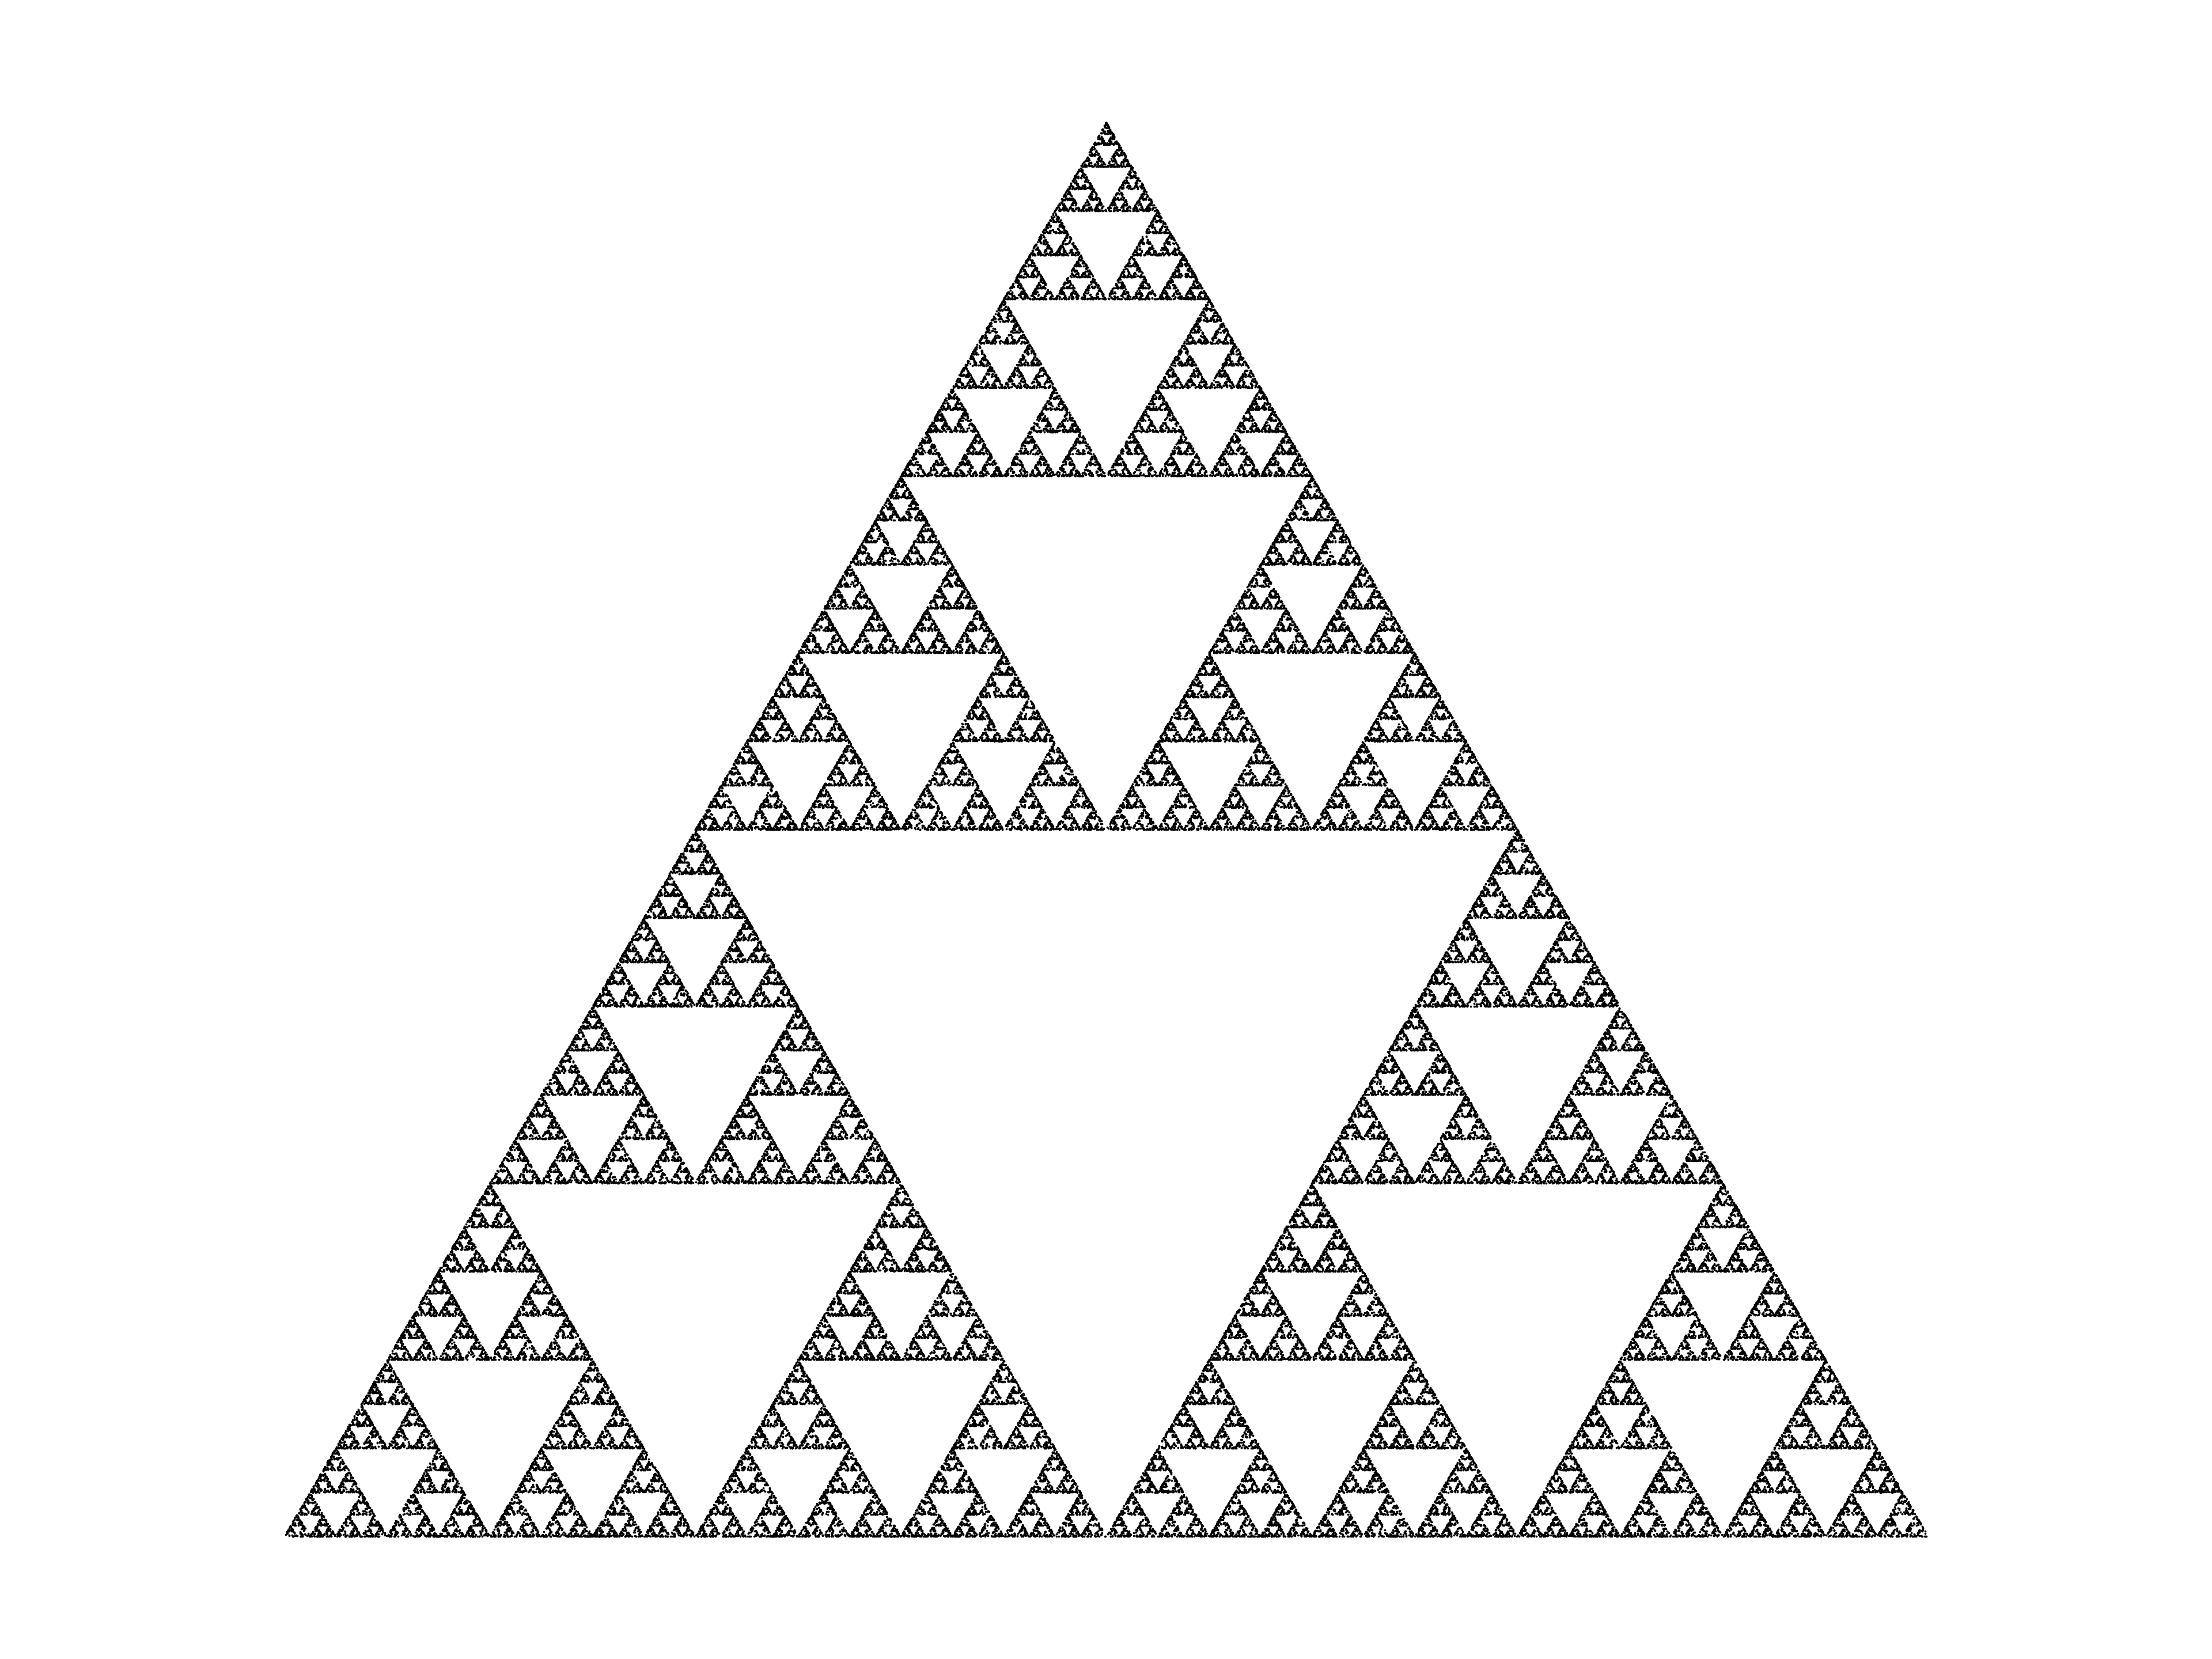
\includegraphics[scale=0.4,trim={1cm 0 1cm 0},clip]{figures-exercices/ifs-02}	
\end{center}

\begin{enumerate}
	\item Soit $(C_k)_{k\in\Nn}$ une suite décroissante (c'est-à-dire $C_{k+1} \subset C_k$) de compacts non vides de $\Rr^n$. 
	Montrer que $C = \bigcap_k C_k$ est un ensemble compact \emph{non vide}.

	\item Soit $T_0$ la zone triangulaire de $\Rr^2$ de sommets $(0,0)$, $(1,0)$, $(\frac12,\frac{\sqrt3}{2})$. Soient les trois transformations affines suivantes :
	$$f_1 \begin{pmatrix}x \\ y \end{pmatrix} = \frac12 \begin{pmatrix}x \\ y \end{pmatrix} \qquad
	f_2\begin{pmatrix}x \\ y \end{pmatrix} = \frac12 \begin{pmatrix}x \\ y \end{pmatrix}+ \begin{pmatrix} \frac12 \\ 0 \end{pmatrix} \qquad
	f_3\begin{pmatrix}x \\ y \end{pmatrix} = \frac12 \begin{pmatrix}x \\ y \end{pmatrix}+ \begin{pmatrix}\frac14 \\ \frac{\sqrt3}{4} \end{pmatrix}
	$$

	On note $T_{n+1} = f_1(T_n) \cup f_2(T_n) \cup f_3(T_n)$.
	\begin{enumerate}
		\item Représenter $T_0$, $T_1$, $T_2$.
		\item Montrer $(T_n)_{n\in\Nn}$ est une suite décroissante de compacts. En déduire que le \emph{triangle de Sierpinski} $T = \bigcap_n T_n$ est un ensemble compact non vide.
		\item Calculer l'aire de $T_n$. Quelle est l'aire de $T$ ?
		\item Calculer le périmètre du bord de $T_n$. Quel est le périmètre du bord de $T$ ?		
	\end{enumerate}	
\end{enumerate}	
\finenonce
\noindication

\correction
\begin{enumerate}
	\item Il faut d'abord comprendre que comme $C_{k+1} \subset C_k$ alors $\bigcap_{1\le k \le n} C_k = C_n$.
	Ainsi $C = \bigcap_k C_k$ est une façon de noter \og$\lim_{k \to + \infty} C_k$\fg.
	
	$C_0$ est par hypothèse un ensemble compact donc fermé et borné.
	Comme $C = \bigcap_{k\in\Nn} C_k \subset C_0$ alors $C$ est un ensemble borné.
	En plus une intersection quelconque d'ensembles fermés est un fermé donc $C$ est un fermé.
	Bilan : $C$ est fermé et borné donc $C$ est compact.
	
	Il reste à montrer que $C$ est non vide.
	Pour chaque $k$, choisissons $x_k\in C_k$. Comme $C_k \subset C$ alors $(x_k)_{k\in\Nn}$ est une suite d'éléments de $C$. Comme $C$ est compact alors $(x_k)_{k\in\Nn}$ admet une sous-suite  $(x_{\phi(k)})_{k\in\Nn}$ convergente. Notons $x_{\infty}$ la limite de cette sous-suite.
	Comme $C$ est fermé alors $x_{\infty} \in C$. Bilan : $C$ est non vide.
	
	\item
	\begin{enumerate}
	\item 	
	Géométriquement la fonction $f_1$ réalise une homothétie de facteur $\frac12$. Ainsi le triangle $T_0$ est réduit d'un facteur $2$ et placé en bas à gauche. Les fonctions $f_2$ et $f_3$ réduisent aussi du même facteur, et ajoutent en plus une translation afin de placer le triangle réduit en bas à droite ou en haut.
	
	%%%%%%%%%%%%%%%%%%%%%%%%%%%%%%%%%%%%%%%%%%%%%%%
	%% Triangle de Sierpinski
	% Les similitudes : shift=translation, scale = homothetie, rotate = angle (en degré)
	\newcommand\simone{\begin{scope}[shift={(0,0)}, scale=.5, rotate=0]}
		\newcommand\simtwo{\begin{scope}[shift={(.5,0)}, scale=.5, rotate=0]}
			\newcommand\simthree{\begin{scope}[shift={(.25,0.433)}, scale=.5, rotate=0]}
				% La figure initiale
				\newcommand\initfigure{\fill (0,0)--++(0:1)--++(120:1)--cycle;}
				%\newcommand\initfigure{\fill (0.5,0.433) circle (1.3cm);}
				%\newcommand\initfigure{\fill (0,0)--++(0,1)--++(1,0)--++(0,-1)--cycle;}
				%\newcommand\initfigure{\fill (0,0)--++(0,0.5)--++(0.5,0)--++(0,-0.5)--cycle;}
				
				% Le programme recursif
				\newcommand{\ifs}[2]{% #1 the counter, #2 the instructions
					\ifnum #1 < 0% stop now
					#2%
					%\relax% Relax, max, on ne fait rien, c'est termine.
					\else%
					\count255=#1%
					\advance\count255 by -1%
					\simone
					\ifs{\number\count255}{#2}                          
				\end{scope}
				
				\simtwo
				\ifs{\number\count255}{#2}                         
			\end{scope}
			
			\simthree
			\ifs{\number\count255}{#2}                         
		\end{scope}
		
		\fi%
	}
	
	\begin{center}
	\begin{tikzpicture}[scale=3]
		\ifs{-1}{\initfigure};
		\node at (0.5,-0.2) {$T_0$};
		
		\draw[->,>=latex, red] (0.80,0.4) to[bend left=20] (1.23,0.25); 
		\draw[->,>=latex, blue] (0.77,0.45) to[bend left=30] (1.72,0.20);
		\draw[->,>=latex, green] (0.75,0.50) to[bend left=40] (1.49,0.70); 
		
		\node[scale=1,red] at (1,0.34) {$f_1$};
		\node[scale=1,blue] at (1,0.55) {$f_2$};    
		\node[scale=1,green] at (1,0.80) {$f_3$}; 
		
		\begin{scope}[xshift=1.1cm]
			\ifs{0}{\initfigure}
			\node at (0.5,-0.2) {$T_1$};
		\end{scope}
		
		
		\begin{scope}[xshift=2.5cm]
			\ifs{1}{\initfigure}
			\node at (0.5,-0.2) {$T_2$};
		\end{scope}
		
		\begin{scope}[xshift=4cm]
			\ifs{2}{\initfigure}
			\node at (0.5,-0.2) {$T_3$};
		\end{scope}
		
		\begin{scope}[scale = 2,xshift=0.7cm, yshift=-1.1cm]
			\ifs{5}{\initfigure}
			\node at (0.5,-0.15) {$T_6$};
		\end{scope}
	\end{tikzpicture}
	\end{center}
	%%%%%%%%%%%%%%%%%%%%%%%%%%%%%%%%%%%%%%%%%%%%%%%
	
		
	Ainsi on peut comprendre le passage de $T_n$ à $T_{n+1}$ de façon additive : on réduit $T_n$ d'un facteur $2$ et on en forme trois copies.
	
	On peut aussi comprendre le passage de $T_n$ à $T_{n+1}$ de façon soustractive : 
	pour chaque triangle (la pointe vers le haut) dans $T_n$ on retire un petit triangle intérieur (la pointe en bas).
	
	Énumération :
	\begin{itemize}
		\item $T_n$ est composé de $3^n$ petits triangles,
		\item chaque petit triangle de $T_n$ a une base de longueur de $\frac{1}{2^n}$.
	\end{itemize}
	
	\item Chaque $T_n$ est un ensemble compact (car borné et fermé en tant qu'union de petits triangles fermés). Par la construction soustractive, il est clair que $T_{n+1} \subset T_n$. Ainsi
	$(T_n)_{n\ge0}$ est une suite décroissante de compacts non vides donc $T = \bigcap_n T_n$ est un compact non vide (voir la première question).

	\item Aire de $T_n$. Chaque petit triangle de $T_n$ est un triangle équilatéral de base $\frac{1}{2^n}$ et donc de hauteur $\frac{\sqrt3}{2} \cdot \frac{1}{2^n}$ ; son aire est  $\frac{\text{base}\times\text{hauteur}}{2} = \frac{\sqrt{3}}{4} \left(\frac{1}{2^n}\right)^2$.
	Ainsi l'aire totale des $3^n$ triangles de $T_n$ est $\mathcal{A}_n =  \frac{\sqrt{3}}{4} \frac{3^n}{4^n}$.
	L'aire de $T$ est la limite de $\mathcal{A}_n$ lorsque $n\to+\infty$, c'est donc $0$.
	
	
	\item Périmètre de $T_n$. 
	Chaque petit triangle de $T_n$ a un périmètre de $3 \frac{1}{2^n}$. 
	Le périmètre total de $T_n$ est donc $\mathcal{L}_n = 3  \frac{3^n}{2^n}$.
	Lorsque $n \to +\infty$, $\mathcal{L}_n \to +\infty$. Donc $T$ a un périmètre infini.
	
	Conclusion : $T$ est un objet géométrique d'aire nulle mais de longueur infinie !
\end{enumerate}	
\end{enumerate}	
\fincorrection

\finexercice


\exercice{}
\enonce[Théorèmes de point fixe]
\sauteligne
\begin{enumerate}
	\item Soit $I=[a,b]$ un intervalle compact de $\Rr$.
	Montrer que toute fonction continue $f : I \to I$ admet au moins un point fixe.
	
	\item Soit $C$ un ensemble compact de $\Rr^n$. Soit $f : C \to C$ une application \emph{quasi-contractante}, c'est-à-dire :
	$$\text{ pour tout } x, y \in C, x \neq y \qquad
	\| f (x) - f (y) \| < \|x - y\|.$$
	Montrer que $f$ admet un unique point fixe.
	(Indication : étudier la fonction $\phi(x) = \|f (x) - x \|$.)

\end{enumerate}
\finenonce

\indication
\begin{enumerate}
	\item Considérer $\psi(x) = f(x)-x$, $\psi(a)$ et $\psi(b)$.
	
	\item Une fonction continue sur un compact...
\end{enumerate}
\finindication

\correction
\begin{enumerate}
	\item Soit $\psi(x) = f(x)-x$. La fonction $\psi$ est continue car $f$ est continue.
	D'une part $\psi(a) = f(a)-a \ge 0$ car $f(a) \in [a,b]$ et d'autre part $\psi(b) = f(b) -b \le 0$ car $f(b) \in [a,b]$. Par le théorème des valeurs intermédiaires, il existe $c \in [a,b]$ tel que $\psi(c)=0$. Pour ce $c$ on a $f(c)-c=0$, soit $f(c)=c$.
	
	\item Unicité. Si $f$ admettait deux points fixes distincts $c$ et $d$, on aurait $\| c - d \| = \|f(c) - f(d) \| < \| c - d \|$, ce qui est impossible.
	
	Existence. La fonction $\phi(x) = \|f (x) - x \|$ est continue de $C$ dans $\Rr^+$ et $C$ est un ensemble compact par hypothèse. En vertu du théorème des valeurs extrêmes, elle atteint
	son minimum en un point $c$. Supposons par l'absurde $\phi(c) > 0$, c’est-à-dire $c \neq f(c)$.
	On aurait $\phi(f(c)) = \| (f \circ f)(c) - f(c) \| <  \| f(c)-c \| = \phi(c)$, contredisant la minimalité de $\phi(c)$. Conclusion : un tel $c$ est bien un minimum pour $\phi$.
\end{enumerate}
\fincorrection
\finexercice


\exercice{}
\enonce[Point de Fermat]
Soit $A, B, C$ trois points du plan. Démontrer qu’il existe un point
$M$ inclus dans le triangle $ABC$ pour lequel la somme des distances $MA + MB + MC$ est minimale.
\finenonce

\indication
On demande de montrer que ce point réalisant le minimum existe, on ne demande pas de trouver sa position.
\finindication


\correction
Notons $\mathcal{T}$ les points du triangle $ABC$ (c'est-à-dire les points intérieurs au triangle et les points du bord du triangle).
Soit $\phi : \mathcal{T} \to \Rr$ la fonction qui à un point $M$ du triangle associe la distance aux trois sommets :
\[ \phi(M) = MA + MB + MC. \]
Une fonction distance, comme $M \mapsto MA =  \| MA \|$, est une fonction continue, car c'est la valeur de la norme (euclidienne).
Ainsi $\phi$ est une fonction continue.
En plus $\mathcal{T}$ est un compact de $\Rr^2$ (car c'est un ensemble fermé et borné).
Par le théorème des valeurs extrêmes, $\phi$ est bornée et atteint ses bornes. En particulier, il existe un point $F \in \mathcal{T}$ tel que $FA+FB+FC$ soit minimal.

Ce point $F$ s'appelle le point de Fermat. Il existe une construction géométrique de ce point.
\fincorrection

\finexercice


\bigskip

Corrections : Arnaud Bodin. Relecture : Axel Renard.

\end{document}
